\documentclass[12pt,letterpaper]{report}
\usepackage{graphicx}

\textwidth 6in

\begin{document}

\title{BAYESIAN OUTPUT ANALYSIS PROGRAM (BOA) VERSION 1.1 USER'S MANUAL}
\author{Brian J. Smith}
\date{January 8, 2005}
\maketitle

\tableofcontents


\chapter{Getting Started}
\noindent


\section{Obtaining BOA}
\noindent BOA is available, in library format, for R and the
Microsoft Windows version of S-PLUS.  The R library is available
from
\begin{center}
http://www.r-project.org
\end{center}
It can be downloaded and installed automatically by entering the
following at the R command line:
\begin{small}
\begin{verbatim}
    > install.packages("boa")
\end{verbatim}
\end{small}
The S-PLUS library is available from
\begin{center}
http://www.public-health.uiowa.edu/boa
\end{center}
To install, extract the BOA zip file to the ``library'' directory
located in the path where S-PLUS is installed.  Once the
appropriate files are installed on your computer, type
\begin{small}
\begin{verbatim}
    > library(boa)
\end{verbatim}
\end{small}
at the R or S-PLUS command line to load the BOA library.


\section{WinBUGS Line Example}
\subsection{Bayesian Model}
\noindent Output from the BUGS Line example is used to illustrate
the capabilities of the BOA program. The Line example involves a
liner regression analysis of the data points (1, 1), (2, 3), (3,
3), (4, 3), and (5, 5). The proposed Bayesian model is
\begin{eqnarray}
\nonumber
   y[i] &\sim& N(mu[i], tau) \\
\nonumber
   mu[i] &=& alpha + beta * (x[i] - mean(x[]))
\end{eqnarray}
with the following priors:
\begin{eqnarray}
\nonumber
   alpha &\sim& N(0, 0.0001) \\
\nonumber
   beta  &\sim& N(0, 0.0001) \\
\nonumber
   tau   &\sim& Gamma(0.001, 0.001)
\end{eqnarray}
Interest lies in estimating the posterior distribution of $alpha$, $beta$,
and $sigma = 1 / \sqrt{tau}$. The starting values for the parameters were varied
to generate two parallel chains from the Markov chain Monte Carlo (MCMC)
sampler. The first chain, line1, was generated with the initial values of
\begin{center}
$alpha$ = -5, $beta$ = 5, $tau$ = 5
\end{center}
whereas, the second chain, line2, was generated with
\begin{center}
$alpha$ = 0.01, $beta$ = 0.01, $tau$ = 0.01
\end{center}


\subsection{WinBUGS Code}
\noindent The code for the Line Example is given below.  The
WinBUGS seed was set to 12345 after loading the initial values.
\begin{small}
\begin{verbatim}
   # Model
   main {
      for(i in 1:N) {
         y[i] ~ dnorm(mu[i], tau)
         mu[i] <- alpha + beta * (x[i] - mean(x[]))
      }

      alpha ~ dnorm(0, 0.0001)
      beta ~ dnorm(0, 0.0001)
      tau ~ dgamma(0.001, 0.001)
   }

   # Data
   list(N = 5, x = c(1, 2, 3, 4, 5), y = c(1, 3,  3, 3, 5))

   # Initial values for first chain
   list(tau = 5, alpha = -5, beta =5)

   # Initial values for second chain
   list(tau = 0.01, alpha = 0.01, beta = 0.01)
\end{verbatim}
\end{small}


\subsection{Saving the WinBUGS Sampler Output}
\noindent In the ``Sampler Monitor Tool'' dialog box $alpha$,
$beta$, and $tau$ were first specified as the nodes.  Then, the
``Update Tool'' dialog box was used to generate two-hundred MCMC
samples for each of the two parallel chains. BOA will import
sampler output saved in the CODA file format.  CODA output can be
generated by entering an asterisk in the Sample Monitor Tool node
list box and pressing the ``coda'' button.  Two windows will
appear - a window with the sampler output and another with the
names of the nodes that were monitored.  The files should be saved
as text files with extensions ``.out'' and ``.ind'', respectively.
Follow the steps below to ensure that WinBUGS saves your CODA
files correctly.
\begin{enumerate}
\item Select the window containing the CODA data to be saved.
\item Choose ``File-$>$Save As...'' from the WinBUGS menu bar to
bring up the ``Save As'' dialog box.
\item Select ``Plain Text (*.txt)'' as the ``Save as type''.
\item Enter the file name enclosed in quotation marks; e.g.
``line1.out'', ``line1.ind'', ``line2.out'', ``line2.ind''.
\item Specify the directory in which to save the file.
\item Press the ``Save'' button to complete the save.
\end{enumerate}
If quotation marks are not used when entering the file names,
Microsoft Windows will automatically append .txt extensions to the
file names when saved.  Carefully follow the previous steps to
avoid import problems in BOA that are a result of CODA file names
with the incorrect extensions.


\subsection{R Line Data}
\noindent The sampler output from the Line Example is included in
the R package.  To load the data type
\begin{small}
\begin{verbatim}
    > data(line)
\end{verbatim}
\end{small}
at the R command line.  Two R data matrices - line1 and line2 -
will be loaded.  These may be imported directly into BOA (see
Section \ref{ssec.datamatrix}).


\chapter{Using the BOA Menu-Driven User Interface}
\noindent
A menu-driven interface is supplied with the BOA. It provides easy access to
all of the command line function. To start the menu system, type
\begin{small}
\begin{verbatim}
    > boa.menu()
\end{verbatim}
\end{small}
to bring up the main menu:
\begin{tiny}
\begin{verbatim}
   Bayesian Output Analysis Program (BOA)
   Version 1.1.3 for i386, mingw32
   Copyright (c) 2004 Brian J. Smith <brian-j-smith@uiowa.edu>

   This program is free software; you can redistribute it and/or
   modify it under the terms of the GNU General Public License
   as published by the Free Software Foundation; either version 2
   of the License or any later version.

   This program is distributed in the hope that it will be useful,
   but WITHOUT ANY WARRANTY; without even the implied warranty of
   MERCHANTABILITY or FITNESS FOR A PARTICULAR PURPOSE.  See the
   GNU General Public License for more details.

   For a copy of the GNU General Public License write to the Free
   Software Foundation, Inc., 59 Temple Place - Suite 330, Boston,
   MA  02111-1307, USA, or visit their web site at
   http://www.gnu.org/copyleft/gpl.html

   NOTE: if the menu unexpectedly terminates, type "boa.menu(recover= TRUE)" to
   restart and recover your work

   BOA MAIN MENU
   *************
   1:File     >>
   2:Data     >>
   3:Analysis >>
   4:Plot     >>
   5:Options  >>
   6:Window   >>
   Selection:
\end{verbatim}
\end{tiny}
Note the message given at startup: if the menu unexpectedly terminates, type
\linebreak ``boa.menu(recover = TRUE)'' to restart and recover your work. There
are a few instances where supplying the wrong type of data will crash the menu
system. Immediately doing a recover will ensure that no data is lost.

\chapter{File Menu}
\noindent
Selecting menu item 1 from the BOA Main Menu brings up the File Menu. Options to
import data, load previously saved session data, save the current session, and
exit the program are available from the File Menu:
\vskip 9pt
\begin{tiny}
\begin{verbatim}
   FILE MENU
   =========
   1:Back
   2:-----------------------+
   3:Import Data         >> |
   4:Load Session           |
   5:Save Session           |
   6:Exit BOA               |
   7:-----------------------+
   Selection:
\end{verbatim}
\end{tiny}

\section{Import Data Menu}
\noindent BOA can import MCMC output from a variety of sources.
Data may be added to the analysis via the import menu at any point
in the analysis.  Three common data formats are supported.
\vskip
9pt
\begin{tiny}
\begin{verbatim}
   IMPORT DATA MENU
   ----------------
   1:Back
   2:---------------------------+
   3:CODA Output Files          |
   4:Flat ASCII File            |
   5:Data Matrix Object         |
   6:View Format Specifications |
   7:Options...                 |
   8:---------------------------+
   Selection:
\end{verbatim}
\end{tiny}

\subsection{Data Options}
\label{ssec.datapar}
\noindent
The Options... menu item lists the values for the user settings used to import
data.
\vskip 9pt
\begin{tiny}
\begin{verbatim}
   Data Parameters
   ===============

   Files
   -----
   1) Working Directory: ""
   2) ASCII File Ext:    ".txt"

   Select parameter to change or press <ENTER> to continue
   1:
\end{verbatim}
\end{tiny}
Most users will want to specify the Working Directory at the start
of their BOA session. This directory should be set to the path in
which the MCMC output files are stored.  The specified working
directory should not be terminated with a slash.

\subsection{CODA Output Files}
\noindent The two CODA output files generated by the Bayesian
inference Using Gibbs Sampling (BUGS or WinBUGS) program can be
imported into BOA. The output file containing the parameter
definitions should be saved as a .ind file; whereas, the file
containing the sampler output should be saved as a .out file. BOA
will expect these files to be located in the Working Directory.
See Section \ref{ssec.datapar} for instructions on specifying the
working directory. Upon choosing to import CODA output the user
will be prompted to
\vskip 9pt
\begin{tiny}
\begin{verbatim}
   Enter filename prefix without the .ind/.out extension [Working
   Directory: "d:/bjsmith/boa"]
   1: line1
\end{verbatim}
\end{tiny}
Only the filename prefix should be specified. BOA will automatically
add the appropriate extensions and load the data from the line1.ind
and line1.out files.

\subsection{Flat ASCII File}
\noindent BOA includes an import filter for general ASCII files.
This is particularly useful for output generated by custom MCMC
programs. The ASCII file should contain one run of the sampler
with the monitored parameters stored in space or tab delimited
columns and with the parameter names in the first row. Iteration
numbers may be specified in a column labeled ``iter''. The ASCII
file should be located in the Working Directory. Upon selected to
import an ASCII file the program will prompt the user to \vskip
9pt
\begin{tiny}
\begin{verbatim}
   Enter filename prefix without the .txt extension [Working Directory:
   "d:/bjsmith/boa/"]
   1: line1
\end{verbatim}
\end{tiny}
Specify only the filename prefix. The import filter will automatically add the
extension and load the data from the line1.txt file. See Section
\ref{ssec.datapar} for instructions on specifying the Working Directory and
the default ASCII file extension.

\subsection{Data Matrix Object}
\label{ssec.datamatrix}
\noindent MCMC output stored as an S
object may be imported into BOA. The object must be a numeric
matrix whose columns contain the monitored parameters from one run
of the sampler. The iteration numbers and parameter names may be
specified in the dimnames. Upon selecting to import a matrix
object the user will be asked to
\vskip 9pt
\begin{tiny}
\begin{verbatim}
   Enter object name [none]
   1: line1
\end{verbatim}
\end{tiny}
BOA will import the data from the line1 object in the current S-PLUS or R
session.

\subsection{View Format Specifications}
\noindent
Selecting this menu item will display the format specifications for the three
types of data that BOA can import.
\vskip 9pt
\begin{tiny}
\begin{verbatim}
   CODA
   - CODA output files produced by WinBUGS (*.ind and  *.out)
   - files must be located in the Working Directory (see  Options)

   ASCII
   - ASCII file (*.txt) containing  the monitored parameters from one run of the
   sampler
   - file must be located in the Working Directory (see  Options)
   - parameters are stored in space or tab delimited  columns
   - parameter names must appear in the first row
   - iteration numbers may be specified in a column  labeled 'iter'

   Matrix Object
   - S or R numeric matrix whose columns contain the  monitored parameters from one
   run of the sampler
   - iteration numbers and parameter names may be  specified in the dimnames
\end{verbatim}
\end{tiny}

\section{Load Session}
\noindent
The Load Session menu item allows users to load previously saved work.
\vskip 9pt
\begin{tiny}
\begin{verbatim}
   Enter name of object to load [none]
   1: line
\end{verbatim}
\end{tiny}

\section{Save Session}
\noindent
All imported data and user settings may be saved at any point in the analysis.
Users will be prompted to
\vskip 9pt
\begin{tiny}
\begin{verbatim}
   Enter name of object to which to save the session data [none]
   1: line
\end{verbatim}
\end{tiny}
The session data will be saved to the specified S object.

\section{Exit BOA}
\noindent
Select this item to exit from the BOA program. Users will be prompted to verify
their intention to exit in order to avoid an unintended termination of the
program.
\vskip 9pt
\begin{tiny}
\begin{verbatim}
   Do you really want to EXIT (y/n) [n]?
   1:
\end{verbatim}
\end{tiny}
Users wishing to save their work should go back and do so before exiting. BOA
will not automatically save the user's work.

\chapter{Data Management Menu}
\noindent
BOA offers a wide range of options for managing the imported data. Two copies of
the data are maintained by the program - the Master dataset and the Working
dataset. The Master dataset is a static copy of the data as it was first
imported. This copy remains essentially unchanged throughout the BOA session.
The Working dataset is a dynamic copy that can be modified by the user. All
analyses are performed on the Working dataset. The Data Management menu offers
the following options:
\vskip 9pt
\begin{tiny}
\begin{verbatim}
   DATA MANAGEMENT MENU
   ====================
   1:Back
   2:---------------------------+
   3:Chains                  >> |
   4:Parameters              >> |
   5:Display Working Dataset    |
   6:Display Master Dataset     |
   7:*****                      |
   8:---------------------------+
   Selection:
\end{verbatim}
\end{tiny}

\section{Chains Menu}
\noindent

\vskip 9pt
\begin{tiny}
\begin{verbatim}
   CHAINS MENU
   -----------
   1:Back
   2:------------+
   3:Combine All |
   4:Delete      |
   5:Subset      |
   6:------------+
   Selection:
\end{verbatim}
\end{tiny}

\subsection{Combine All Chains}
\noindent
Selecting this options will combine together all of the chains in the Working
dataset. Sequencing is preserved by concatenating together the different chains
and then ordering the result by the iteration numbers in the original chains.
Note that this may result in a chain with multiple samples at a given iteration.
The resulting chain contains only those parameters common to all chains.

CAUTION: Although possible to do so, convergence diagnostics and
autocorrelations should not be computed for combined chains.  A combined chain
is essentially a single chain with potentially multiple samples per iteration.
These analyses expect that a single chain has no more than one sample per
iteration.

\subsection{Delete Chain}
\noindent
Chains may be discarded when they are no longer needed. Discarding chains may
free up a substantial amount of computer memory. The program prompts the user to
select the chain(s) to discard.
\vskip 9pt
\begin{tiny}
\begin{verbatim}
   DELETE CHAINS
   =============

   Chains:
   -------

      1       2
   "line1" "line2"

   Specify chain index or vector of indices [none]
   1:
\end{verbatim}
\end{tiny}
The specified chain(s) will be immediately deleted from the Master dataset. If
the Working dataset has not been modified, the chain(s) will be deleted from
there as well. If modifications were made to the Working dataset, the user can
copy the new Master dataset to the Working dataset via the Reset option. If no
chain is entered at the prompt, no action is taken.

\subsection{Subset Chains}
\noindent
Subsets of the MCMC sequences can be selected for analysis via the Subset
option.
\vskip 9pt
\begin{tiny}
\begin{verbatim}
   SUBSET WORKING DATASET
   ======================
   Specify the indices of the items to be included in the subset.
   Alternatively, items may be excluded by supplying negative indices.
   Selections should be in the form of a number or numeric vector.

   Chains:
   -------

         1       2
   "line1" "line2"

   Specify chain indices [all]
   1: c(1,2)

   Parameters:
   -----------

         1      2       3
   "alpha" "beta" "tau"

   Specify parameter indices [all]
   1: -2

   Iterations:
   +++++++++++

         Min Max Sample
   line1   1 200    200
   line2   1 200    200

   Specify iterations [all]
   1: 50:200
\end{verbatim}
\end{tiny}
In this example, both chains were first included in the subset. Since the
default is to include all chains, this line could have been left blank. Next,
the $beta$ parameter is excluded by supplying a negative sign in front of the
selection. Finally, the subset is limited to iteration 50-200. Users can verify
that the subset was successfully constructed by selecting the option to display
the Working dataset (output not shown).

\noindent
{\bf Thinning:} Thinning refers to the practice of including every $k^{th}$
iteration from a chain. Users can thin a chain by using the {\it seq} function
when prompted to specify the iterations. For example, the following input will
included every other iteration from the chain:
\vskip 9pt
\begin{tiny}
\begin{verbatim}
   seq(1, 200, length = 100)
\end{verbatim}
\end{tiny}
A description of the {\it seq} function can be found at the end of the Appendix.

\section{Parameters Menu}
\noindent

\vskip 9pt
\begin{tiny}
\begin{verbatim}
   PARAMETERS MENU
   ---------------
   1:Back
   2:-----------+
   3:Set Bounds |
   4:Delete     |
   5:New        |
   6:-----------+
   Selection:
\end{verbatim}
\end{tiny}

\subsection{Set Parameter Bounds}
\noindent
This option allows the user to specify the lower and upper bounds (support) of
selected MCMC parameters. The parameter support factors into the computation of
the Brooks, Gelman \& Rubin convergence diagnostics.
\vskip 9pt
\begin{tiny}
\begin{verbatim}
   SET PARAMETER BOUNDS
   ====================

   Chains:
   -------

         1       2
   "line1" "line2"

   Specify chain index or vector of indices [all]
   1:

   Parameters:
   -----------

         1       2       3
   "alpha"  "beta" "tau"

   Specify parameter index or vector of indices [all]
   1: 3

   Specify lower and upper bounds as a vector [-Inf, Inf]
   1: c(0, Inf)
\end{verbatim}
\end{tiny}
In this example, the variance parameter $tau$ has been restricted to only
non-negative values. When no chain(s) is specified, the default is to apply the
change to all of the chains. Likewise, the default is to select all parameters
and to set the bounds to $(-\infty, \infty)$.

\subsection{Delete Parameters}
\noindent
Often times it may be desired to delete parameters that are not of interest in
the analysis.  This may arise in cases where data other than model parameters
were saved to the output file imported into BOA. Alternatively, the user may
only be interested in functions of the original parameters.  Once the new
parameter is created using the methods described in the following section, the
unnecessary parameter upon which it is based may be deleted.  Deleted parameters
will speed up the manipulation of data in BOA.
\vskip 9pt
\begin{tiny}
\begin{verbatim}
   DELETE PARAMETERS
   =================

   Parameters:
   -----------

         1       2       3
   "alpha"  "beta" "tau"

   Specify parameter index or vector of indices [none]
   1:
\end{verbatim}
\end{tiny}

\subsection{Create New Parameters}
\noindent
BOA includes an option to create new parameters.  Most S functions can be used
to create the new parameter.  Typically, a new parameter is defined as a
function of the existing parameters.  For instance, suppose the user was
interested in analyzing the standard deviation $sigma = 1 / \sqrt{tau}$.  The
following menu commands demonstrate how to create this new parameter:
\vskip 9pt
\begin{tiny}
\begin{verbatim}
   NEW PARAMETER
   =============

   Common Parameters:
   ------------------

   [1] "alpha" "beta"  "tau"

   New parameter name [none]
   1: sigma
   Read 1 items

   Define the new parameter as a function of the parameters listed above
   1: 1 / sqrt(tau)
   Read 1 items
\end{verbatim}
\end{tiny}
$sigma$ has now been added to the two datasets in BOA and will be available to all
subsequent analyses.

\section{Display Master Dataset}
\noindent
Selecting this option will display summary information for the Master dataset.
\vskip 9pt
\begin{tiny}
\begin{verbatim}
   CHAIN SUMMARY INFORMATION:
   ==========================

   Iterations:
   +++++++++++

         Min Max Sample
   line1   1 200    200
   line2   1 200    200

   Support: line1
   --------------

      alpha beta tau sigma
   Min  -Inf -Inf   0     0
   Max   Inf  Inf Inf   Inf

   Support: line2
   --------------

      alpha beta tau sigma
   Min  -Inf -Inf   0     0
   Max   Inf  Inf Inf   Inf
\end{verbatim}
\end{tiny}

\section{Reset}
\noindent
The Reset option copies the Master dataset to the Working dataset. This undoes
any modifications that were made to the Working dataset.

\chapter{Analysis Menu}
\noindent
The statistical analysis procedures are accessible through the Analysis
Menu. Analyses are categorized into two groups -- Descriptive Statistics
and Convergence Diagnostics.
\vskip 9pt
\begin{tiny}
\begin{verbatim}
   ANALYSIS MENU
   =============
   1:Back
   2:---------------------------+
   3:Descriptive Statistics  >> |
   4:Convergence Diagnostics >> |
   5:Options...                 |
   6:---------------------------+
   Selection:
\end{verbatim}
\end{tiny}

\section{Descriptive Statistics Menu}
\noindent
Options to compute autocorrelations, cross-correlations, and summary statistics
are available from the Descriptive Statistics Menu.
\vskip 9pt
\begin{tiny}
\begin{verbatim}
   DESCRIPTIVE STATISTICS MENU
   ---------------------------
   1:Back
   2:---------------------------------------+
   3:Autocorrelations                       |
   4:Correlation Matrix                     |
   5:Highest Probability Density Intervals  |
   6:Summary Statistics                     |
   7:---------------------------------------+
   Selection:
\end{verbatim}
\end{tiny}

\subsection{Autocorrelations}
\noindent
This option produces lag-autocorrelations for the monitored parameters within
each chain. High autocorrelations indicate slow mixing within a chain and,
usually, slow convergence to the posterior distribution.
\vskip 9pt
\begin{tiny}
\begin{verbatim}
   LAGS AND AUTOCORRELATIONS:
   ==========================

   Chain: line1
   ------------

               Lag 1      Lag 5       Lag 10      Lag 50
   alpha -0.10005297 0.04361973  0.001152681 -0.06391649
   beta   0.07166133 0.10149584 -0.059398063  0.07936142
   tau    0.32327917 0.06211792 -0.064798232  0.01946111
   sigma  0.42629373 0.11736382 -0.103620199 -0.11424204
\end{verbatim}
\end{tiny}
Option 11 in Section \ref{sec.analysispar} allows the user to set the lags at
which autocorrelations are computed.

\subsection{Correlation Matrix}
\noindent
This option returns the correlation matrix for the parameters in each chain.
High correlation among parameters may lead to slow convergence to the posterior.
Associated models may need to be reparameterized in order to reduce the amount
of cross-correlation.
\vskip 9pt
\begin{tiny}
\begin{verbatim}
   CROSS-CORRELATION MATRIX:
   =========================

   Chain: line1
   ------------

         alpha      beta       tau      sigma
   alpha 1
   beta  0.1643217  1
   tau   -0.0556438 -0.0416541 1
   sigma 0.0937184  0.0422862  -0.66123 1
\end{verbatim}
\end{tiny}

\subsection{Highest Probability Density Intervals}
\noindent
Highest probability density (HPD) interval estimation is one means of generating
Bayesian posterior intervals. HPD intervals span a region of values containing
$(1 - \alpha) \times 100\%$ of the posterior density such that the posterior
density within the interval is always greater than that outside. Consequently,
HPD intervals are of the shortest length of any of the Bayesian intervals. The
algorithm described by Chen and Shao (1999) is used to compute the HPD
intervals in BOA under the assumption of unimodal marginal posterior
distributions.  The alpha level for the intervals can be modified through Option
12 in Section \ref{sec.analysispar}.
\vskip 9pt
\begin{tiny}
\begin{verbatim}
   HIGHEST PROBABILITY DENSITY INTERVALS:
   ======================================

   Alpha level = 0.05

   Chain: line1
   ------------

         Lower Bound Upper Bound
   alpha   1.9470000    3.937000
   beta    0.1762000    1.491000
   tau     0.0618500    5.767000
   sigma   0.3347497    2.074796
\end{verbatim}
\end{tiny}

\subsection{Summary Statistic}
\noindent
This option prints summary statistics for the parameters in each chain. The
sample mean and standard deviation are given in the first two columns. These are
followed by three separate estimates of the standard error: 1) a naive estimate
(the sample standard deviation divided by the square root of the sample size)
which assumes the sampled values are independent, 2) a time--series estimate
(the square root of the spectral density variance estimate divided by the sample
size) which gives the asymptotic standard error (Geweke, 1992), and 3) a batch
estimate calculated as the sample standard deviation of the means from
consecutive batches of size 50 divided by the square root of the number of
batches. The autocorrelation between batch means follows and should be close to
zero. If not, the batch size should be increased. Quantiles are given after the
batch autocorrelation. Finally, the minimum and maximum iteration numbers and
the total sample size round out the table.
\vskip 9pt
\begin{tiny}
\begin{verbatim}
   SUMMARY STATISTICS:
   ===================

   Batch size for calculating Batch SE and (Lag 1) ACF = 50

   Chain: line1
   ------------

            Mean        SD   Naive SE   MC Error   Batch SE  Batch ACF     0.025
   alpha 3.0214700 0.5210029 0.03684047 0.07251309 0.04842256 -0.7384625 2.0480500
   beta  0.8120946 0.3519652 0.02488770 0.07171012 0.01329908 -0.7084603 0.2435375
   tau   1.9402362 1.8348540 0.12974377 0.15531429 0.18201157 -0.3526486 0.2042925
   sigma 0.9987152 0.5574588 0.03941829 0.07653543 0.06009981  0.2221603 0.3932961
               0.5    0.975 MinIter MaxIter Sample
   alpha 3.0115000 4.378725       1     200    200
   beta  0.7870000 1.555925       1     200    200
   tau   1.3480000 6.465950       1     200    200
   sigma 0.8613953 2.214427       1     200    200
\end{verbatim}
\end{tiny}
Options 13 and 14 in Section \ref{sec.analysispar} allow the user to change
the batch size and the quantiles, respectively.  See the Appendix for
instructions on setting the number of significant digits and display width.

\section{Convergence Diagnostics Menu}
\noindent
The Convergence Diagnostics Menu offers the user the following diagnostic
methods:
\vskip 9pt
\begin{tiny}
\begin{verbatim}
   CONVERGENCE DIAGNOSTICS MENU
   ----------------------------
   1:Back
   2:-----------------------+
   3:Brooks, Gelman & Rubin |
   4:Geweke                 |
   5:Heidelberger & Welch   |
   6:Raftery & Lewis        |
   7:-----------------------+
   Selection:
\end{verbatim}
\end{tiny}
These are the most commonly used methods used to asses the convergence of MCMC
output. A brief explanation of each approach is given in the following sections.
Users are referred to the work of Brooks and Roberts (1998) and Cowles and
Carlin (1996) for a more in-depth review and comparison of these methods.

\subsection{Brooks, Gelman \& Rubin Convergence Diagnostic}
\label{ssec.bandg}
\noindent
The code for implementing the Gelman and Rubin (1992) convergence diagnostic in
BOA is based on the {\it itsim} function contributed to the Statlib archive by
Andrew Gelman (http://lib.stat.cmu.edu).

The Brooks, Gelman and Rubin convergence diagnostic is appropriate for the
analysis of two or more parallel chains, each with different starting values
which are overdispersed with respect to the target distribution. Several methods
for generating starting values for the MCMC samplers have been proposed (Gelman
and Rubin, 1992; Applegate et al., 1990; Jennison, 1993). The following
diagnostic information was obtained for the line example:
\vskip 9pt
\begin{tiny}
\begin{verbatim}
   BROOKS, GELMAN AND RUBIN CONVERGENCE DIAGNOSTICS:
   =================================================

   Iterations used = 101:200

   Potential Scale Reduction Factors
   ---------------------------------

      alpha      beta       tau
   0.9962501 1.0019511 1.0099913

   Multivariate Potential Scale Reduction Factor = 1.010112

   Corrected Scale Reduction Factors
   ---------------------------------

         Estimate    0.975
   alpha 1.107170 1.116686
   beta  1.087270 1.131090
   tau   1.027212 1.090423
\end{verbatim}
\end{tiny}
The diagnostic originally proposed by Gelman and Rubin (1992) is based on a
comparison of the within and between chain variance for each variable. This
comparison is used to estimate the {\it potential scale reduction factor} (PSRF)
-- the multiplicative factor by which the sampling-based estimate of the scale
parameter of the marginal posterior distribution might be reduced if the chains
were run to infinity. To adjust for the sampling variability in the variance
estimates, the correction proposed by Brooks and Gelman (1998) is applied to the
PSRF to produce the {\it corrected scale reduction factor} (CSRF). BOA also
displays an upper quantile of the sampling distribution for the CSRF. Users can
control which quantile is computed via Option 1 in Section
\ref{sec.analysispar}. Brooks and Gelman (1998) developed a multivariate
extension to the PSRF known as the {\it multivariate potential scale reduction
factor} (MPSRF). The MPSRF does not include a correction for sampling
variability. This statistic is relevant when interest lies in general
multivariate functionals of the chain. The MPSRF and the PSRF satisfy the
following relationship:
\begin{displaymath}
   max(\mbox{PSRF}) \le \mbox{MPSRF}
\end{displaymath}
Computation of the reduction factors is based on analysis of variance and
sampling from the normal distribution. To avoid violations of the latter
assumption, BOA transforms any parameters specified to be restricted to the
range (a, b) to the logarithmic or logit scale before calculating this
diagnostic. By default only the second half of the chains (iterations 101-200)
is used to compute the reduction factors. Option 2 in \ref{sec.analysispar}
can be used to vary the proportion of samples from the end of the chains to be
included in the analysis. If the estimates are approximately equal to one (or,
as a rule of thumb, the 0.975 quantile is $\le$ 1.2), the samples may be
considered to have arisen from the stationary distribution. In this case,
descriptive statistics may be calculated for the combined latter 50\% of
iterations from all of the chains.

\subsection{Geweke Convergence Diagnostic}
\label{ssec.geweke}
\noindent
The Geweke convergence diagnostic is appropriate for the analysis of individual
chains when convergence of the {\it mean} of some function of the sampled
parameters is of interest. The following diagnostic information was obtained for
the line example:
\vskip 9pt
\begin{tiny}
\begin{verbatim}
   GEWEKE CONVERGENCE DIAGNOSTIC:
   ==============================

   Fraction in first window = 0.1
   Fraction in last window = 0.5

   Chain: line1
   ------------

               alpha       beta        tau
   Z-Score -0.1226878 -0.1306432 -0.9944621
   p-value  0.9023544  0.8960575  0.3199980
\end{verbatim}
\end{tiny}
The chain is divided into two ``windows'' containing a set fraction of the first
and the last iterations. Options 3 and 4 in Section \ref{sec.analysispar}
allow the user to set the fraction of iterations included in the first and the
last window, respectively. Geweke (1992) proposed a method to compare the mean
of the sampled values in the first window to the mean of the sampled values in
the last window. There should be a sufficient number of iterations between the
two windows to reasonably assume that the two means are approximately
independent. His method produces a {\it Z} statistic calculated as the
difference between the two means divided by the asymptotic standard error of
their difference, where the variance is determined by spectral density
estimation. As the number of iterations approaches infinity, the {\it Z}
statistic approaches the $N(0,1)$ if the chain has converged. {\it Z} values
which fall in the extreme tails of the $N(0,1)$ suggest that the chain in the
first window had not fully converged. The two-sided p-value outputted by BOA
gives the tail probability associated with the observed {\it Z} statistic. It is
common practice to conclude that there is evidence against convergence when the
p-value is less than 0.05. Otherwise, it can be said that the results of this
test do not provide any evidence against convergence. This does not, however,
prove that the chain has converged.

\subsection{Heidelberger and Welch Convergence Diagnostic}
\noindent
The Heidelberger and Welch convergence diagnostic is appropriate for the
analysis of individual chains. The following diagnostic information was obtained
for the line example:
\vskip 9pt
\begin{tiny}
\begin{verbatim}
   HEIDLEBERGER AND WELCH STATIONARITY AND INTERVAL HALFWIDTH TESTS:
   =================================================================

   Halfwidth test accuracy = 0.1

   Chain: line1
   ------------

         Stationarity Test Keep Discard     C-von-M Halfwidth Test      Mean
   alpha            passed  200       0 0.037295593         passed 3.0214700
   beta             passed  200       0 0.008893071         failed 0.8120946
   tau              passed  200       0 0.126287673         failed 1.9402362
         Halfwidth
   alpha 0.1421230
   beta  0.1405493
   tau   0.3044104
\end{verbatim}
\end{tiny}
Heidelberger and Welch's (1983) stationarity test is based on Brownian bridge
theory and uses the Cramer-von-Mises statistic. If there is evidence of
non-stationarity, the test is repeated after discarding the first 10\% of the
iterations. This process continues until the resulting chain passes the test or
more than 50\% of the iterations have been discarded. BOA reports the number of
iterations that were kept, the number of iterations that were discarded, and the
Cramer-von-Mises statistic. Failure of the chain to pass this test indicates
that a longer run of the MCMC sampler is needed in order to achieve
convergence.

A halfwidth test is performed on the portion of the chain that passes the
stationarity test for each variable. Spectral density estimation is used to
compute the asymptotic standard error of the mean. If the halfwidth of the
confidence interval for the mean is less than a specified fraction (accuracy) of
this mean, the halfwidth test indicates that the mean is estimated with
acceptable accuracy. The confidence level and accuracy can be modified through
Options 5 and 6, respectively, in Section \ref{sec.analysispar}. Failure of
the halfwidth test implies that a longer run of the MCMC sampler is needed to
increase the accuracy of the estimated posterior mean.

\subsection{Raftery and Lewis Convergence Diagnostic}
\noindent
The Raftery and Lewis convergence diagnostic is appropriate for the analysis of
individual chains. The following diagnostic information was obtained for the
line example:
\vskip 9pt
\begin{tiny}
\begin{verbatim}
   RAFTERY AND LEWIS CONVERGENCE DIAGNOSTIC:
   =========================================

   Quantile = 0.025
   Accuracy = +/- 0.02
   Probability = 0.9

   Chain: line1
   ------------

         Thin Burn-in Total Lower Bound Dependence Factor
   alpha    1       2   160         165          0.969697
   beta     1       5   188         165          1.139394
   sigma    1       2   160         165          0.969697
\end{verbatim}
\end{tiny}
The diagnostic proposed by Raftery and Lewis (1992b) tests for convergence to
the stationary distribution and estimates the run-lengths needed to accurately
estimate quantiles of functions of the parameters. The user may specify the
quantile of interest, the desired degree of accuracy in estimating this
quantile, and the probability of attaining the indicated degree of accuracy.
Options 7, 9, and 10 in Section \ref{sec.analysispar} allow the user to
modify these quantities. BOA computes the ``lower bound'' -- the number of
iterations needed to estimate the specified quantile to the desired accuracy
using independent samples.  If fewer iterations than this bound have been loaded
into BOA, the following warning is displayed:
\vskip 9pt
\begin{tiny}
\begin{verbatim}
   ******* Warning *******
   Available chain length is 200.
   Re-run simulation for at least 3746 iterations
   OR reduce the quantile, accuracy, or probability to be estimated.
\end{verbatim}
\end{tiny}
If sufficient MCMC iterations are available, BOA lists the lower bound, the
total number of iterations needed for each parameter, the number of initial
iterations to discard as the burn-in set, and the thinning interval to be used.
The dependence factor measures the multiplicative increase in the number of
iterations needed to reach convergence due to within-chain correlation.
Dependence factors greater than 5.0 often indicate convergence failure and a
need to reparameterize the model (Raftery and Lewis, 1992a).

\section{Analysis Options}
\label{sec.analysispar}
\noindent

\vskip 9pt
\begin{tiny}
\begin{verbatim}
   Analysis Parameters
   ===================

   Brooks, Gelman & Rubin
   ----------------------
   1)  Alpha Level:       0.05
   2)  Window Fraction:   0.5

   Geweke
   ------
   3)  Window 1 Fraction: 0.1
   4)  Window 2 Fraction: 0.5

   Heidelberger & Welch
   --------------------
   5)  Accuracy:          0.1
   6)  Alpha Level:       0.05

   Raftery & Lewis
   ---------------
   7)  Accuracy:          0.005
   8)  Alpha Level:       0.05
   9)  Delta:             0.001
   10) Quantile:          0.025

   Statistics
   ----------
   11) ACF Lags:          c(1, 5, 10, 50)
   12) Alpha Level:       0.05
   13) Batch Size:        50
   14) Quantiles:         c(0.025, 0.5, 0.975)
\end{verbatim}
\end{tiny}

\chapter{Plot Menu}
\noindent
Like the Analysis Menu, the Plot Menu categorizes the available plots into a
Descriptive and Convergence Diagnostic group. Most of the options found under
the Analysis Menu have a counterpart within the Plot Menu.
\vskip 9pt
\begin{tiny}
\begin{verbatim}
   PLOT MENU
   =========
   1:Back
   2:---------------------------+
   3:Descriptive             >> |
   4:Convergence Diagnostics >> |
   5:Options...                 |
   6:---------------------------+
   Selection:
\end{verbatim}
\end{tiny}

\section{Descriptive Plot Menu}
\noindent

\vskip 9pt
\begin{tiny}
\begin{verbatim}
   DESCRIPTIVE PLOT MENU
   ---------------------
   1:Back
   2:-----------------+
   3:Autocorrelations |
   4:Density          |
   5:Running Mean     |
   6:Trace            |
   7:-----------------+
   Selection:
\end{verbatim}
\end{tiny}

\pagebreak

\subsection{Autocorrelations Plot}
\noindent
Plot the first several lag-autocorrelations for each parameter in each chain.

\begin{figure}[h]
\centering
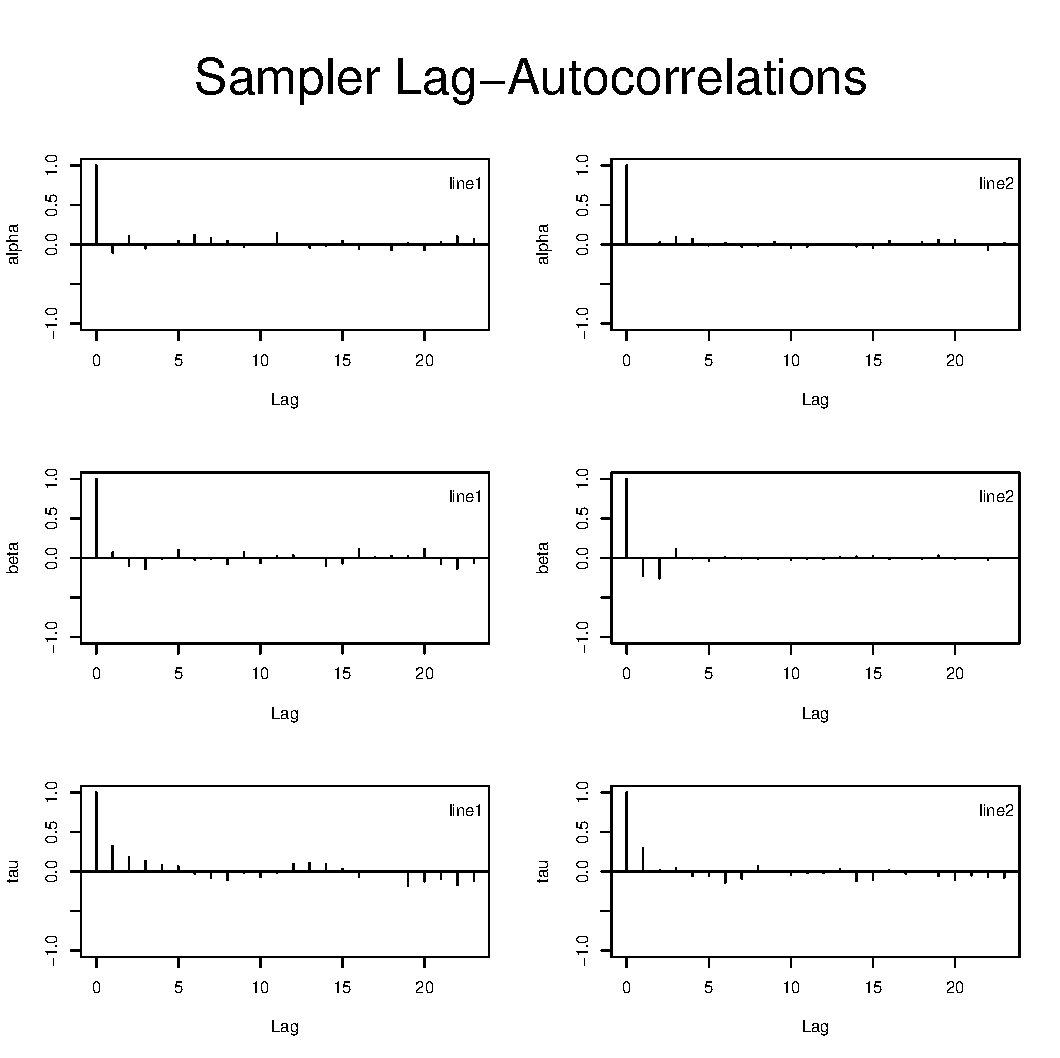
\includegraphics[keepaspectratio,width=5in]{autocorr.pdf}
\end{figure}

\pagebreak

\subsection{Density Plot}
\noindent
Plot the kernel density estimate for each parameters in each
chain. Options 3 and 4 in Section \ref{sec.plotpar} control the width and
type of window used in the computations, respectively.

\begin{figure}[h]
\centering
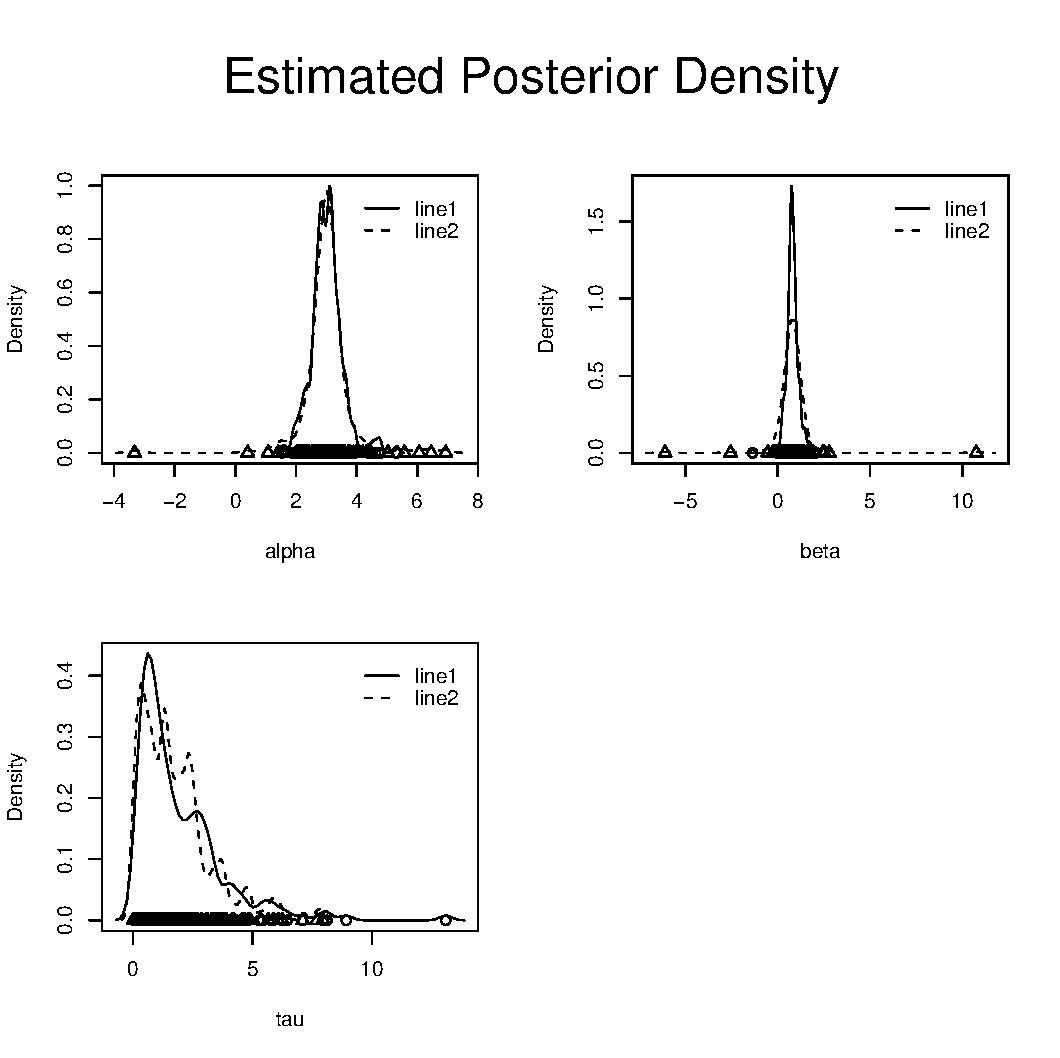
\includegraphics[keepaspectratio,width=5in]{density.pdf}
\end{figure}

\pagebreak

\subsection{Running Mean Plot}
\noindent
Generate a time series plot of the running mean for each parameter in each
chain. The running mean is computed as the mean of all sampled values up to and
including that at a given iteration.

\begin{figure}[h]
\centering
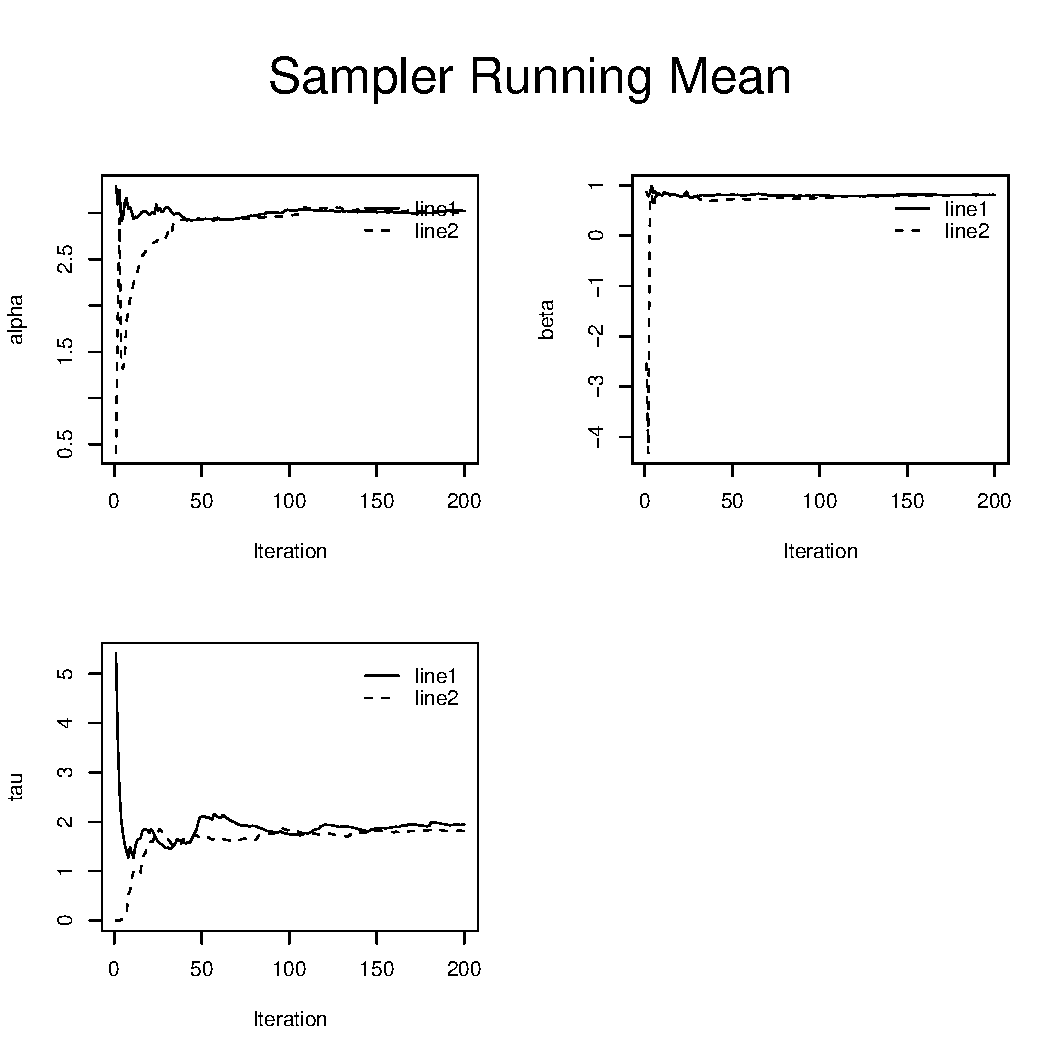
\includegraphics[keepaspectratio,width=5in]{mean.pdf}
\end{figure}

\pagebreak

\subsection{Trace Plot}
\noindent
Generate a time series plot of the sampled points for each parameter in each
chain.

\begin{figure}[h]
\centering
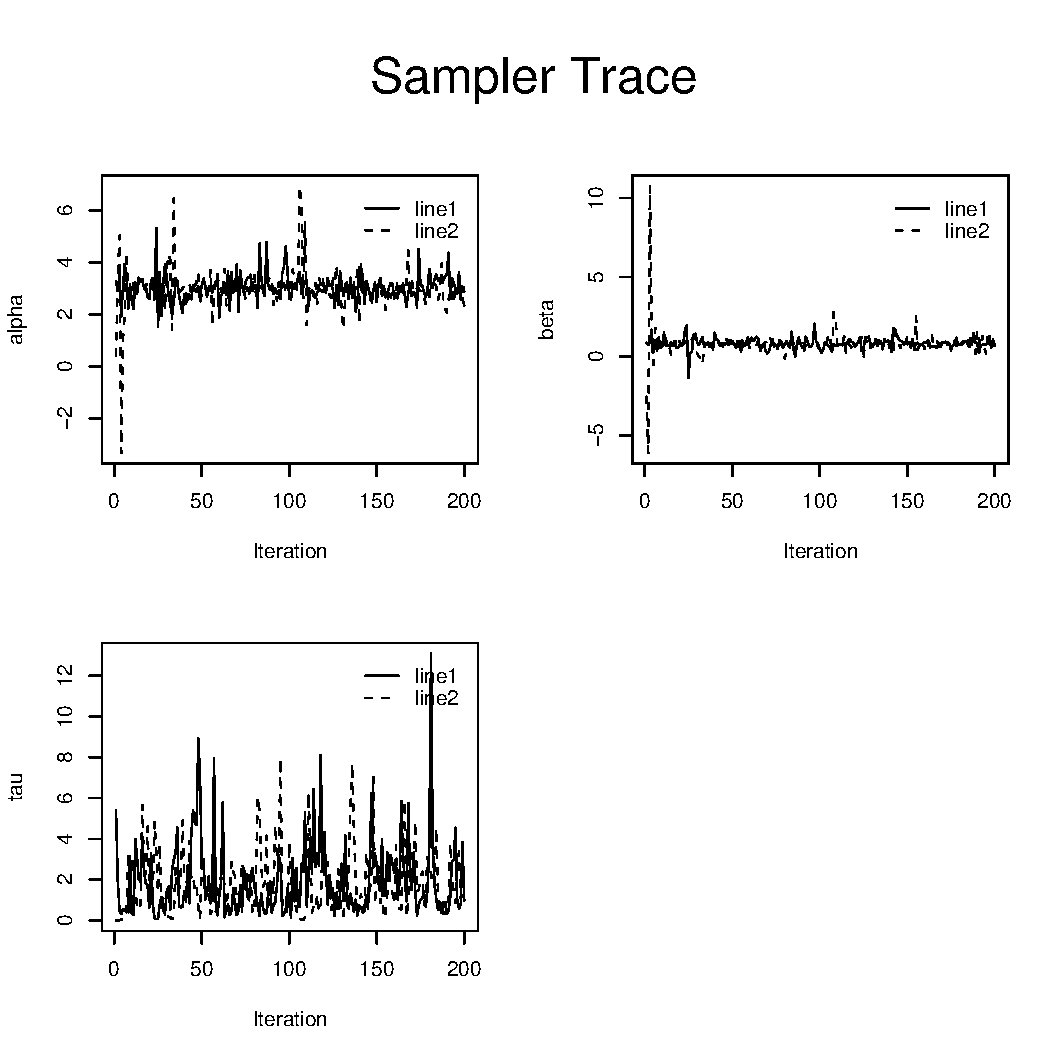
\includegraphics[keepaspectratio,width=5in]{trace.pdf}
\end{figure}

\pagebreak

\section{Convergence Diagnostics Plot Menu}
\noindent

\vskip 9pt
\begin{tiny}
\begin{verbatim}
   CONVERGENCE DIAGNOSTICS PLOT MENU
   ---------------------------------
   1:Back
   2:----------------+
   3:Brooks & Gelman |
   4:Gelman & Rubin  |
   5:Geweke          |
   6:----------------+
   Selection:
\end{verbatim}
\end{tiny}

\pagebreak

\subsection{Brooks and Gelman Plot}
\noindent
Plots the Brooks and Gelman {\it multivariate potential scale reduction factor}
and the maximum of the {\it potential scale reduction factors} (see Section
\ref{ssec.bandg}) for successively larger segments of the chains. The first
segment contains the first 50 iterations in the chains. The remaining iterations
are then partitioned into equal bins and added incrementally to construct the
remaining segments. Option 1 in Section \ref{sec.plotpar} governs the number
of bins used for the plot. Scale factors are plotted against the maximum
iteration number in the segments. Cubic splines are used to interpolate through
the point estimates from the segments.

\begin{figure}[h]
\centering
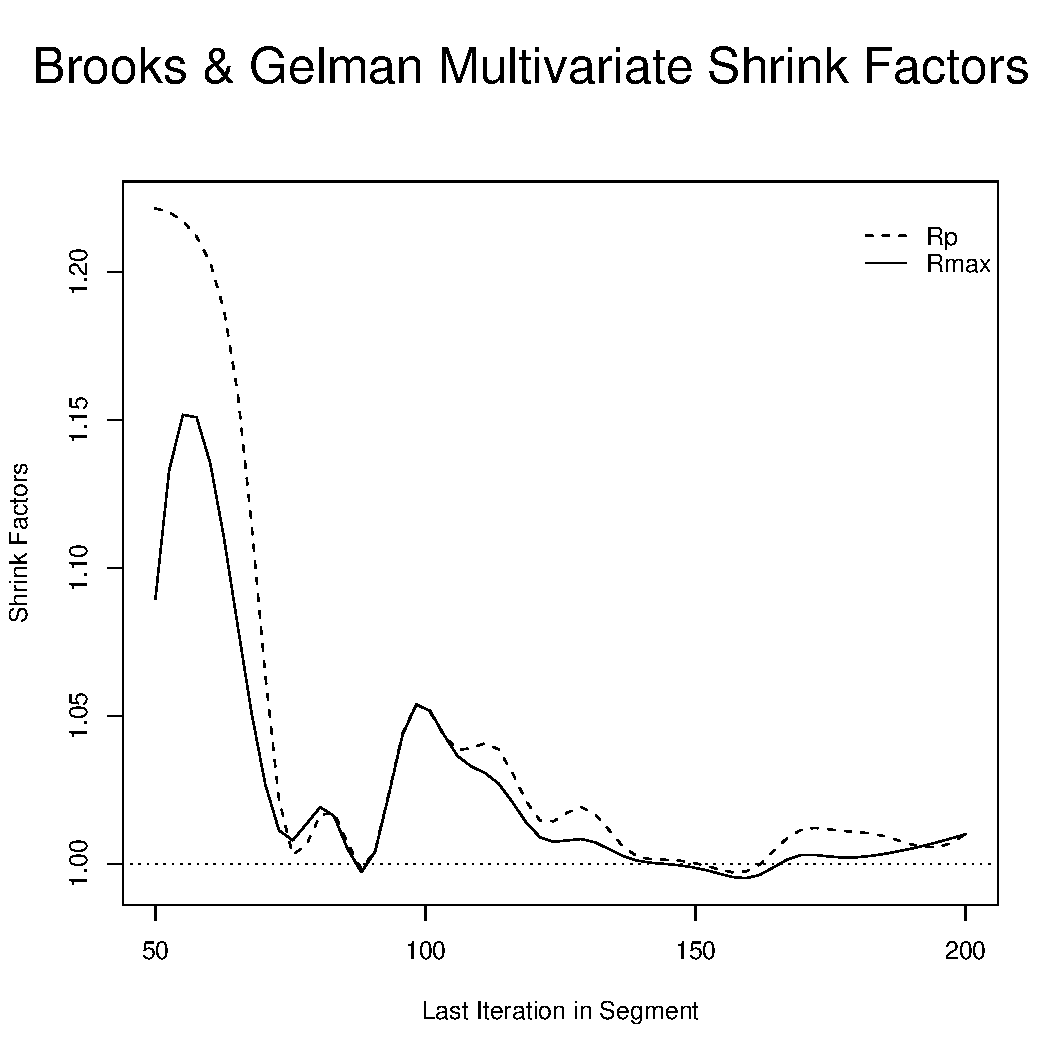
\includegraphics[keepaspectratio,width=5in]{bandg.pdf}
\end{figure}

\pagebreak

\subsection{Gelman and Rubin Plot}
\noindent
Plots the Gelman and Rubin {\it corrected potential scale reduction factors}
(see Section \ref{ssec.bandg}) for each parameter in successively larger
segments of the chain. The first segment contains the first 50 iterations in the
chain. The remaining iterations are then partitioned into equal bins and added
incrementally to construct the remaining segments. Options 5 and 6 in Section
\ref{sec.plotpar} control the error rate for the upper quantile and the number
of bins, respectively. Option 7 determines the proportion of samples from the
end of the chains to be included in the analysis. The scale factor is plotted
against the maximum iteration number for the segment. Cubic splines are used to
interpolate through the point estimates from the segments.

\begin{figure}[h]
\centering
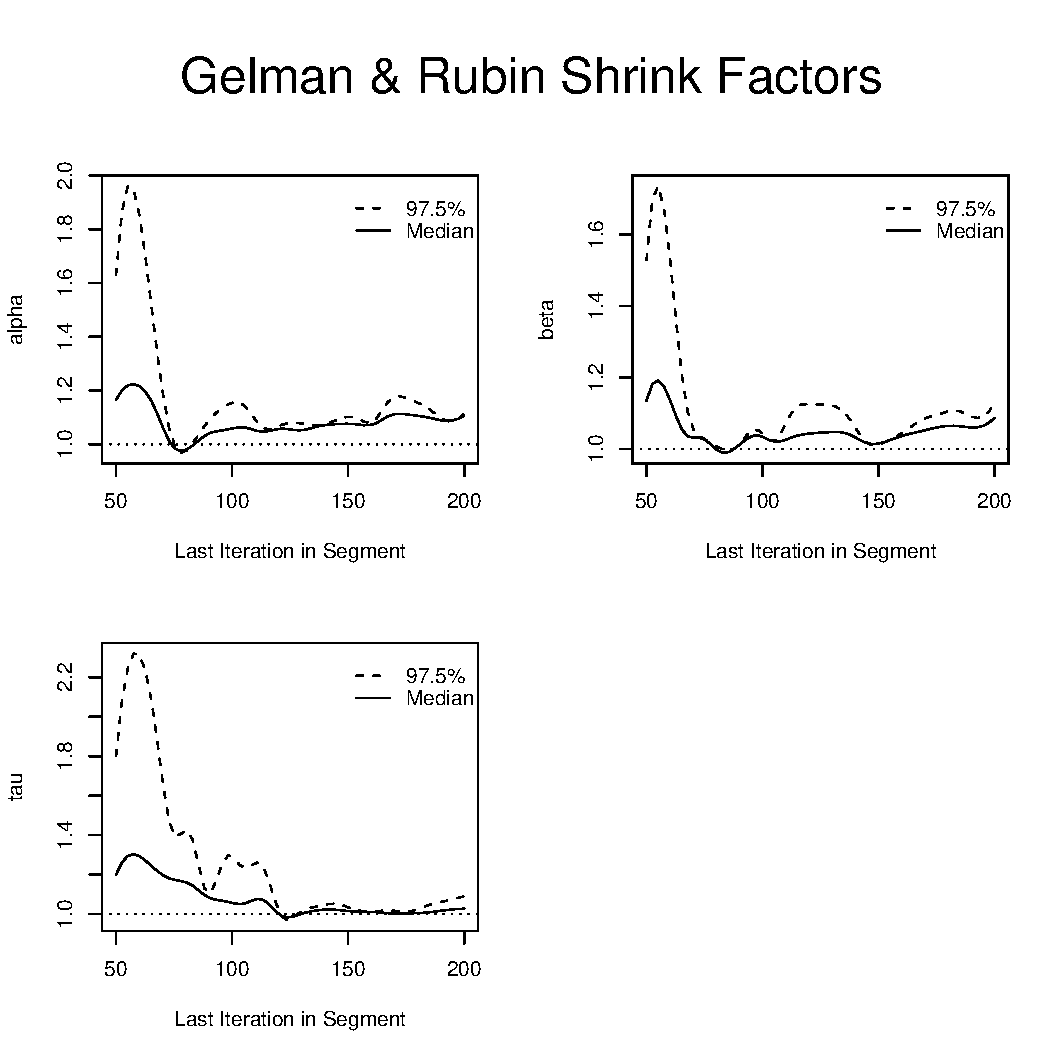
\includegraphics[keepaspectratio,width=5in]{gandr.pdf}
\end{figure}

\pagebreak

\subsection{Geweke Plot}
\noindent
Plots the Geweke Z statistic (see Section \ref{sec.plotpar}) for each
parameter in successively smaller segments of the chain. The $k^{th}$ segment
contains the last ((number of bins - k + 1) / number of bins)*100\% of the
iterations in the chain. Options 8 and 9 in Section \ref{sec.plotpar} set
the error rate for the confidence bounds and the number of bins included in the
plot, respectively. Options 10 and 11 control the fraction of iterations covered
by the windows used in computing the Geweke diagnostic. It may be possible that
some of the subsets contain too few iterations to compute the test statistic.
Such segments, if they exist, are automatically omitted from the plot. The test
statistic is plotted against the minimum iteration number for the segment.

\begin{figure}[h]
\centering
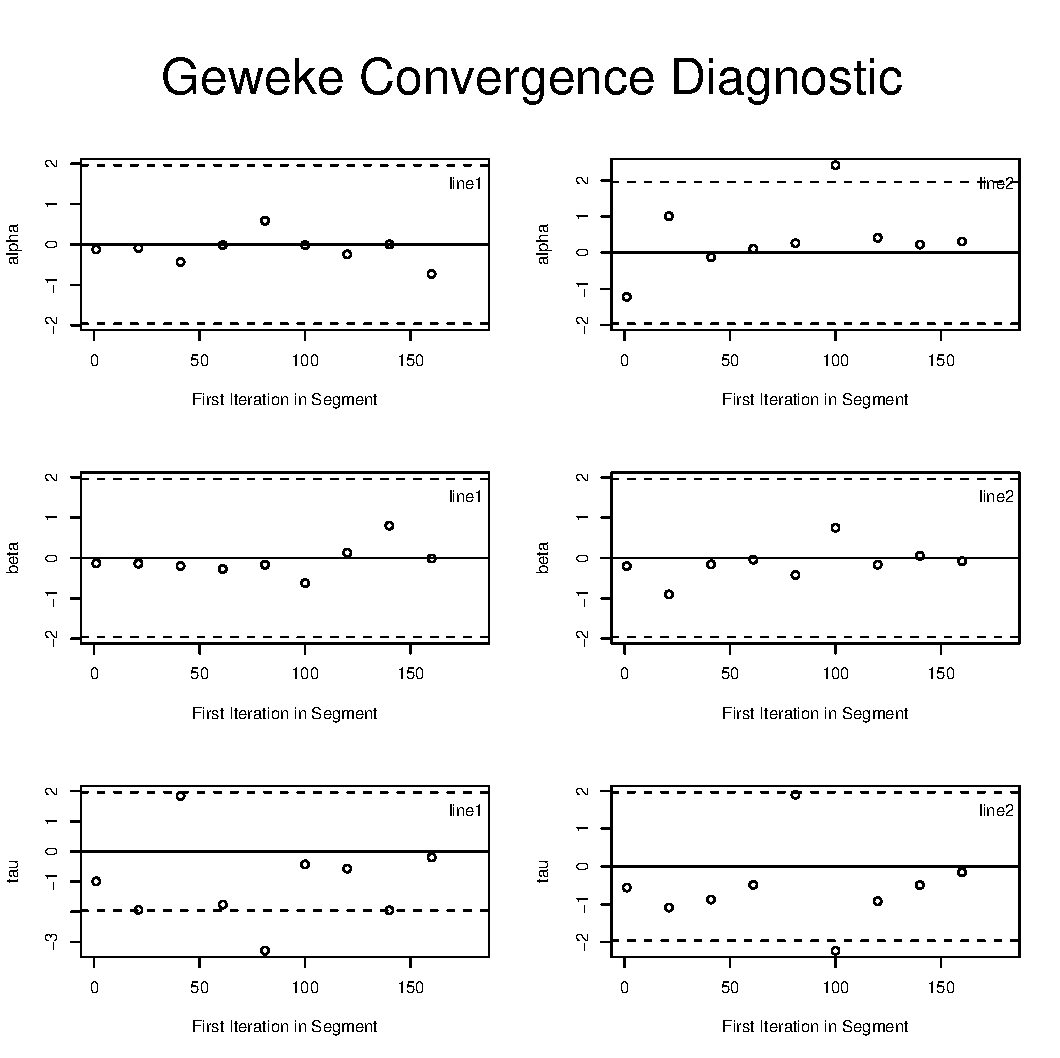
\includegraphics[keepaspectratio,width=5in]{geweke.pdf}
\end{figure}

\pagebreak

\section{Plot Options}
\label{sec.plotpar}
\noindent

\vskip 9pt
\begin{tiny}
\begin{verbatim}
   Plot Parameters
   ===============

   Brooks & Gelman
   ---------------
   1)  Number of Bins:      20
   2)  Window Fraction:     0.5

   Density
   -------
   3)  Bandwidth:           function (x)
                           0.5 * diff(range(x))/(log(length(x)) + 1)
   4)  Kernel:              "gaussian"

   Gelman & Rubin
   --------------
   5)  Alpha Level:         0.05
   6)  Number of Bins:      20
   7)  Window Fraction:     0.5

   Geweke
   ------
   8)  Alpha Level:         0.05
   9)  Number of Bins:      10
   10) Window 1 Fraction:   0.1
   11) Window 2 Fraction:   0.5

   Graphics
   --------
   12) Legend:                 TRUE
   13) Title:                  TRUE
   14) Keep Previous Plots:    FALSE
   15) Plot Layout:            c(3, 2)
   16) Plot Chains Separately: FALSE

   Select parameter to change or press <ENTER> to continue
   1:
\end{verbatim}
\end{tiny}
The options grouped under the Graphics heading control the general layout used
to generate plots. The following gives a brief description of each of these
options:
\begin{description}
\item[12)] If set to ``TRUE'' legends are included in the plots; otherwise, a
value of ``FALSE'' will suppress plot legends.
\item[13)] If set to ``TRUE'' titles are added to the plots; otherwise, a
value of ``FALSE'' will suppress plot titles.
\item[14)] If set to ``TRUE'' all plots generated in BOA will be kept open; otherwise,
a value of ``FALSE'' indicates that only the most recently opened plots be kept
open.
\item[15)] The number of rows and columns, respectively, of plots to display in one
graphics window.
\item[16)] If set to ``TRUE'' only one chain is displayed per plot; otherwise, a value
of ``FALSE'' forces all of the chains to be displayed on the same plot.
\end{description}

\chapter{Options Menu}
\noindent
The Options Menu serves as a central location from which the options in Sections
\ref{ssec.datapar}, \ref{sec.analysispar}, and \ref{sec.plotpar} can be
accessed.
\vskip 9pt
\begin{tiny}
\begin{verbatim}
   GLOBAL OPTIONS MENU
   ===================
   1:Back
   2:------------+
   3:Analysis... |
   4:Data...     |
   5:Plot...     |
   6:All...      |
   7:------------+
   Selection:
\end{verbatim}
\end{tiny}

\chapter{Window Menu}
\noindent
The Window Menu allows the user to switch between and save the active graphics
windows.
\vskip 9pt
\begin{tiny}
\begin{verbatim}
   WINDOW 2 MENU
   =============
   1:Back
   2:------------------------+
   3:Previous                |
   4:Next                    |
   5:Save to Postscript File |
   6:Close                   |
   7:Close All               |
   8:------------------------+
   Selection:
\end{verbatim}
\end{tiny}
The number of the active graphics window is displayed in the title of his menu.
In this example, graphics window 1 is the active window.

\section{Previous Graphics Window}
\noindent
Make the previous graphics window in the list of open windows the active
graphics window.

\section{Next Graphics Window}
\noindent
Make the next graphics window in the list of open windows the
active graphics window.

\section{Save to Postscript File}
\noindent
Saves the active graphics window to a postscript file. The user is prompted to
enter the name of the postscript file in which to save the contents of the
graphics window.
\vskip 9pt
\begin{tiny}
\begin{verbatim}
   Enter name of file to which to save the plot [none]
   1:
\end{verbatim}
\end{tiny}
Only the name of the file should be given. The file will be automatically saved
in the Working Directory (see Section \ref{ssec.datapar}). Microsoft Windows
users may save the graphics window in other formats directly from the S-PLUS or
R program menus.

\section{Close Graphics Window}
\noindent
Close the active graphics window.

\section{Close All Graphics Window}
\noindent
Closes all open graphics windows.

\chapter{S-PLUS and R Basics}
\noindent

\section{Output Display Options}
\noindent
The {\it options} function in S-PLUS and R can be used to control the format of
the outputted text in BOA. This should be done prior to starting BOA. To set the
number of significant digits to be displayed, type
\vskip 9pt
\begin{tiny}
\begin{verbatim}
   options(digits = <value>)
\end{verbatim}
\end{tiny}
The number of characters allowed per line can be controlled by entering the
command
\vskip 9pt
\begin{tiny}
\begin{verbatim}
   options(width = <value>)
\end{verbatim}
\end{tiny}

\section{Vectors in S}
\noindent
Several menu selections in BOA prompt the user to input a vector of data.
Vectors in S can be supplied in a variety of ways. The simplest way to construct
a vector is with the concatenation function {\it c}:
\vskip 9pt
\begin{tiny}
\begin{verbatim}
   c(<element 1>, <element 2>, ..., <element n>)
\end{verbatim}
\end{tiny}
where the elements may be numerical or logical values or character
strings. Another means of constructing vectors is with the {\it seq}
function:
\vskip 9pt
\begin{tiny}
\begin{verbatim}
   seq(<starting value>, <ending value>, length = <number of values>)
\end{verbatim}
\end{tiny}
or
\vskip 9pt
\begin{tiny}
\begin{verbatim}
   seq(<starting value>, <ending value>, by = <step size>)
\end{verbatim}
\end{tiny}
where ``length'' is number of values in the vector and ``by'' is the spacing
between successive values in the vector. The ``:'' operator, which is a special
case of the {\it seq} function, can also be used to construct vectors. This
operator can be defined as
\vskip 9pt
\begin{tiny}
\begin{verbatim}
   <starting value>:<ending value>
      = seq(<starting value>, <ending value>, by = 1)
\end{verbatim}
\end{tiny}
For more detailed information about these functions, consult the help systems in
S-PLUS or R.

\begin{thebibliography}{99}
\bibitem{} Applegate, D., Kannan, R. and Polson, N.G. (1990). Random
polynomial time algorithms for sampling from joint distributions.
{\it Technical report no. 500, Carnegie-Mellon University}.

\bibitem{} Brooks, S. and Gelman, A. (1998). General methods for monitoring
convergence of iterative simulations. {\it Journal of Computational and
Graphical Statistics}, {\bf 7(4)}, 434-455.

\bibitem{} Brooks, S.P. and Roberts, G.O. (1998). Convergence assessment
techniques for Markov chain Monte Carlo. {\it Statistics and Computing},
{\bf 8(4)}, 319-335.

\bibitem{} Cowles, M.K. and Carlin, B.P. (1996). Markov chain Monte Carlo
convergence diagnostics: a comparative review. {\it Journal of the American
Statistical Association}, {\bf 91}, 883-904.

\bibitem{} Gelman, A. and Rubin, D.B. (1992). Inference from iterative
simulation using multiple sequences. {\it Statistical Science}, {\bf 7},
457-511.

\bibitem{} Geweke, J. (1992). Evaluating the accuracy of sampling-based
approaches to calculating posterior moments. In {\it Bayesian
Statistics 4}, eds. J.M. Bernardo, J.O. Berger, A.P. Dawid and
A.F.M. Smith. Oxford: Oxford University Press.

\bibitem{} Heidelberger, P. and Welch, P. (1983). Simulation run length
control in the presence of an initial transient. {\it Operations Research},
{\bf 31}, 1109-1144.

\bibitem{} Jennison, C. (1993). Discussion of ``Bayesian computation via
the Gibbs sampler and related Markov chain Monte Carlo methods.''
by Smith and Roberts, {\it Journal of the Royal Statistical Society,
Series B}, {\bf 55}, 54-56.

\bibitem{} Raftery, A. L. and Lewis, S. (1992a). Comment: One long run with
diagnostics: implementation strategies for Markov chain Monte Carlo.
{\it Statistical Science}, {\bf 7}, 493-497.

\bibitem{} Raftery, A. L. and Lewis, S. (1992b). How many iterations in the
Gibbs sampler? In {\it Bayesian Statistics 4}, eds. J.M. Bernardo, J.O.
Berger, A.P. Dawid and A.F.M. Smith. Oxford: Oxford University Press.
\end{thebibliography}

\end{document}
